\chapter{Understanding SSL/TLS}
Let's start off with some basics and a bit of history. SSL is the ``Secure 
Sockets Layer'' and was first developed by Netscape Communications. Later the 
protocol was standardised by the IETF\footnote{The Internet Engineering Task 
Force or IETF, is an organisation that publishes many of the standards relevant 
to SSL/TLS. The standards are published in the form of documents known as RFCs. 
The most significant of these from our perspective are RFC6101 (SSL3.0), 
RFC2246 (TLS1.0), RFC4346 (TLS1.1) and RFC5246 (TLS1.2)} and was renamed to TLS 
(Transport Layer Security).

The purpose of SSL/TLS is to secure the communications between two parties. The
initiating  party is known as the ``client'' and the responding party is known
as the ``server''. The term ``secure'' here covers authentication,
confidentiality and integrity. In other words an attacker should not be able 
to:
\begin{itemize}
\item fool a party into believing that they are someone else;
\item eavesdrop and hence learn the content of messages being exchanged; or
\item modify those messages without being detected.
\end{itemize}

There are limits to the security that is provided by the protocol; for example
there is no  provision for preventing an attacker from learning that two parties
are engaging in communications and their associated IP addresses. Nor does it
prevent an attacker from learning the approximate size of messages transferred.

There are multiple versions of SSL/TLS:
\begin{itemize}
\item SSL 1.0. This version was developed by Netscape but was never publicly 
released due to fundamental security flaws.
\item SSL 2.0. This was the first publicly released version of the protocol. It 
was first published in February 1995, but is no longer in common usage due to 
significant security issues. OpenSSL 1.1.0 no longer supports this version.
\item SSL 3.0. This was the last version of the protocol developed by Netscape 
and represented a significant change from version 2.0. All subsequent versions 
were based on this version. It should no longer be used although there are 
still some servers on the internet which only support this version.
\item TLS 1.0. The first version of the protocol published by the IETF. In 
practice this is very similar to SSL 3.0, although one of the major differences 
is the support for \emph{extensions}.
\item TLS 1.1. Published in 2006 this provided a number of security tweaks.
\item TLS 1.2. Published in 2008 this version provided some significant changes
including  support for authenticated encryption ciphers.
\end{itemize}

The protocol provides the capability for the two parties to negotiate between 
them which version of the protocol will be used. For example if the client 
supports all versions up to TLS 1.2, but the server only supports versions up 
to TLS 1.0, then version negotiation will take place and agree on the highest 
available version that both support (in this case TLS 1.0).

\section{Establishing Identity}

In order to authenticate a remote party there has to be a system in place for 
reliably establishing and verifying the identify of that party. Most commonly 
SSL/TLS only authenticates the server not the client, i.e. from a server's 
perspective the identity of the client is unknown, but the client is able to 
confirm that they are talking to the server that they think they are (and not a 
malicious attacker pretending to be that server). Frequently higher level 
application protocols may add the capability to authenticate clients, although
it is also possible to do it at the SSL/TLS layer if so desired.

Identity is established through the use of a \emph{digital certificate}. The 
digital certificate provides public data about a server for which it is issued. 
For example, the certificate will contain the hostname(s) for which it is 
valid. In order to obtain a certificate a server operator must first create a 
private and a public key. The private key must remain secret. Loss of the 
private key would be catastrophic to the security of the system. Anyone with 
access to the private key can masquerade as the server. The public key is 
mathematically related to the private key, although it is not possible to 
derive the private key from it. The public key is published in the digital 
certificate and it is safe for this to be available to everyone.

Having obtained a private/public key pair a server operator must obtain their
certificate from a \emph{Certificate Authority} (CA)\footnote{CAs can be
privately run and purely internal to an organisation; or they could be public.
Which type is most appropriate will depend on what the certificte will be used
for. There are many public CAs available. A simple search in your search engine
of choice should turn up lots of links. Many, but not all, charge a fee for
issuing a certificate.}. The CA will, at a minimum, verify that the server 
operator is in control of the domain name to be included in the certificate. 
Dependant on the type of certificate ordered, other checks may also be 
performed to verify the identity of the server operator. Finally the CA will 
issue the certificate which itself will be digitally signed by the CA.

Both the digital certificate, and the associated private key are installed on 
the SSL/TLS server. When a client accesses the server, the server will send 
its certificate back to the client. In order for authentication to be
successful the client must verify two things:
\begin{enumerate}
\item The certificate provided by the server is valid and issued by a CA that 
the client trusts.
\item The server has the private key corresponding to the public key published 
in the certificate.
\end{enumerate}

Part of the role of the SSL/TLS protocol is to enable the client to perform the 
above checks during the establishment of a connection. If either of these 
checks fail then the connection will fail.

As mentioned above it is also possible for the server to authenticate the 
client as part of the SSL/TLS protocol. If this capability is used then it works
in a very similar way  to that described above. The primary difference is that
the client will also have to create a private/public key pair and obtain a
digital certificate from a CA that the server trusts. 

\section{Ciphersuites}

SSL/TLS itself does not mandate the use of any particular cryptographic 
algorithms. Instead it provides a framework for combining different algorithms 
together and enabling the client and server to negotiate between them which 
combination of algorithms will be used to protect messages that are exchanged. 
A group of algorithms combined in this way is known as a \emph{ciphersuite}. 
There are many different ciphersuites that are available\footnote{At the time 
of writing OpenSSL 1.1.0 supports 168 different ciphersuites}. Each
ciphersuite identifies a set of algorithms that it will use to satsify the 
following cryptographic primitives:
\begin{itemize}
\item Authentication. What algorithm will be used to digitally sign various 
aspects of the communication in order to establish and verify the identify of
the parties (either just the server, or both the server and the client). The 
algorithm used here will be the same one used to generate the public/private 
key pair associated with the digital certificate. Examples of common algorithms 
include RSA, DSA and ECDSA.
\item Key Exchange. Typically a new encryption key will be generated for each
connection. Do not confuse this encryption key with the public/private key pair
associated with the digital certificate. The encryption key must be shared
between both ends of the communication and must be \emph{private} to prevent an
eavesdropper from being able to decrypt messages. Key exchange algorithms solve 
the problem of how two parties will agree on a key without enabling an 
eavedropper to work out what it is. Examples of algorithms that are used for 
this purpose include RSA, DH and ECDH.\footnote{You will also very
frequently come across the so-called ``ephemeral'' variants of DH and ECDH
known as DHE and ECHDE respectively.}
\item Encryption. Having established a shared encryption key, the two 
communicating parties can start to protect their communications from 
eavesdroppers by encrypting the data that they exchange. Examples of common 
encryption algorithms include AES, CAMELLIA and ChaCha20.
\item Integrity. The algorithm used to protect communications from being 
tampered with by an attacker. Often the algorithm used here will be one known 
as HMAC combined with a message digest algorithm such as SHA256 or SHA512. A
message digest is simply a secure ``hash'' function. They take arbitrary 
length input data and output a fixed length ``hash'' value that exhibits 
certain security properties (including that it is not possible to derive the 
input data from the hash output). Alternatively, integrity could be provided by
a \emph{mode} of the underlying  encryption cipher. Modes are a complex topic,
but in essence define the manner in which an encryption algorithm is used.
Examples of modes that provide integrity include GCM and CCM.
\end{itemize}

To look at some example ciphersuites you can use the \lstinline!openssl ciphers!
command line tool:
\begin{verbatim}
$ openssl ciphers -v
\end{verbatim}

The \lstinline!-v! argument here instructs OpenSSL to display verbose output.
Without any other arguments this will list information about the DEFAULT
ciphersuites (i.e. those ciphersuites that are available unless you configure
OpenSSL differently).

\begin{lstlisting}[float=tb,label=lst:ciphers-extract,caption=An
extract from \lstinline!openssl ciphers -v! output]
ECDHE-ECDSA-AES256-GCM-SHA384 TLSv1.2 Kx=ECDH     Au=ECDSA Enc=AESGCM(256) Mac=AEAD
ECDHE-RSA-AES256-GCM-SHA384 TLSv1.2 Kx=ECDH     Au=RSA  Enc=AESGCM(256) Mac=AEAD
DHE-RSA-AES256-GCM-SHA384 TLSv1.2 Kx=DH       Au=RSA  Enc=AESGCM(256) Mac=AEAD
ECDHE-ECDSA-CHACHA20-POLY1305 TLSv1.2 Kx=ECDH     Au=ECDSA Enc=CHACHA20/POLY1305(256) Mac=AEAD
ECDHE-RSA-CHACHA20-POLY1305 TLSv1.2 Kx=ECDH     Au=RSA  Enc=CHACHA20/POLY1305(256) Mac=AEAD
DHE-RSA-CHACHA20-POLY1305 TLSv1.2 Kx=DH       Au=RSA  Enc=CHACHA20/POLY1305(256) Mac=AEAD
ECDHE-ECDSA-AES128-GCM-SHA256 TLSv1.2 Kx=ECDH     Au=ECDSA Enc=AESGCM(128) Mac=AEAD
ECDHE-RSA-AES128-GCM-SHA256 TLSv1.2 Kx=ECDH     Au=RSA  Enc=AESGCM(128) Mac=AEAD
DHE-RSA-AES128-GCM-SHA256 TLSv1.2 Kx=DH       Au=RSA  Enc=AESGCM(128) Mac=AEAD
ECDHE-ECDSA-AES256-SHA384 TLSv1.2 Kx=ECDH     Au=ECDSA Enc=AES(256)  Mac=SHA384
ECDHE-RSA-AES256-SHA384 TLSv1.2 Kx=ECDH     Au=RSA  Enc=AES(256)  Mac=SHA384
DHE-RSA-AES256-SHA256   TLSv1.2 Kx=DH       Au=RSA  Enc=AES(256)  Mac=SHA256
ECDHE-ECDSA-AES128-SHA256 TLSv1.2 Kx=ECDH     Au=ECDSA Enc=AES(128)  Mac=SHA256
ECDHE-RSA-AES128-SHA256 TLSv1.2 Kx=ECDH     Au=RSA  Enc=AES(128)  Mac=SHA256
DHE-RSA-AES128-SHA256   TLSv1.2 Kx=DH       Au=RSA  Enc=AES(128)  Mac=SHA256
ECDHE-ECDSA-AES256-SHA  TLSv1 Kx=ECDH     Au=ECDSA Enc=AES(256)  Mac=SHA1
ECDHE-RSA-AES256-SHA    TLSv1 Kx=ECDH     Au=RSA  Enc=AES(256)  Mac=SHA1
\end{lstlisting}

An extract of the output from \lstinline!openssl ciphers -v! is given in 
Listing \ref{lst:ciphers-extract}. The columns tell you the following
information:
\begin{itemize}
\item The ciphersuite name such as \lstinline!ECDHE-ECDSA-AES256-CCM8!.
\item The earliest protcol version that the ciphersuite is available from. Note 
that ciphersuites are \emph{forward compatible}. Therefore if a ciphersuite is
marked as \lstinline!SSLv3! then it is compatible with all protocol versions 
from SSL 3.0 right up to TLS 1.2.
\item The key exchange algorithm used by the ciphersuite (\lstinline!Kx! here 
stands for ``Key Exchange'').
\item The algorithm being used to provide authentication (\lstinline!Au!).
\item The encryption (\lstinline!Enc!) algorithm.
\item The algorithm being used to provide integrity. This will either be a 
message digest that is being used in conjunction with the HMAC algorithm, or it
will indicate that integrity is being provided by a mode of the encryption 
cipher (\lstinline!AEAD!).
\end{itemize}

\section{Records}

Data is transferred between clients and servers using \emph{records}. Think of 
a record as being like an envelope containing data. The envelope has some basic 
information about its contents written on it, such as:
\begin{itemize}
\item The amount of data that is being transferred
\item The type of data that is being transferred
\end{itemize}

The record will also apply any cryptographic operations to the data that may be 
appropriate dependant on the current state of the connection. During initial 
connection various parameters need to be agreed between the two parties to 
determine exactly what cryptographic operations will be applied. One of these 
parameters is the ciphersuite. The ciphersuite that is currently in use will 
define the encryption that is to be applied to the data within the record.

As well as the encrypted data the record will also contain a Message 
Authentication Code (MAC). The MAC utilises the integrity algorithm and a 
secret key, shared between the two parties, to calculate a code that is unique
to the data being sent. Any attempt by an attacker to modify the data will mean
that the MAC code will fail to verify when it is checked by the remote party 
and the connection will be aborted.

Optionally records can also compress the data that they transmit. This is done 
prior to encryption. This is usually not done in practice due to security 
concerns associated with this capability.

\section{The Handshake}

The initial exchange of messages during which cryptographic parameters are 
exchanged is known as the \emph{handshake}. While making the initial connection
no crypotgraphic parameters will have yet been agreed. Therefore there is no
encryption and no MAC on individual records.  Record data is sent in
\emph{plaintext}. For this reason the protocol has been designed such that no
application data is sent until the connection has been established and
cryptographic parameters have been agreed. A MAC of the entire set of handshake 
messages is calculated and verified at the last step of the handshake process. 
In this way, even though inidividual records do not have integrity protection, 
the handshake as a whole does.

Handshake messages are transmitted between the client and server in rec-ords. A 
single record may contain multiple handshake messages, or a single handshake 
message may be spread across multiple records. A handshake is always initiated 
by a client sending a ``ClientHello'' message to a server. A typical handshake 
is shown in figure \ref{fig:typical-hand}.

\begin{figure}[t]
\fbox{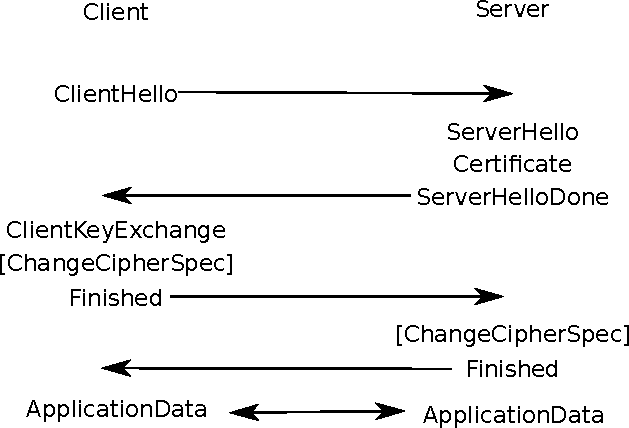
\includegraphics[width=0.9\textwidth]{devel-tls/understand-tls/typicalhand.pdf}}
\caption{A typical SSL/TLS handshake.}
\label{fig:typical-hand}
\end{figure}

The ClientHello contains:
\begin{itemize}
\item The highest protocol version supported by the client.
\item Some random data generated by the client.
\item The id of a pre-existing session that the client wishes to use (if any).
\item A list of the ciphersuites the client is willing to use.
\item A list of the compression methods the client is willing to use (if any).
\item A list of \emph{extensions} the client supports.
\end{itemize}

There are quite a few different messages possible and not all messages will 
always be sent. Some messages are optional and may depend on the ciphersuite 
chosen; whether the client is required to provide a certificate; etc. The 
handshake shown in figure \ref{fig:typical-hand} is an example of a full 
handshake. Once a client has completed its first handshake with a server it can 
usually reuse the cryptographic parameters negotiated so that it does not need 
to go through a second or subsequent full handshake. Instead it performs an 
\emph{abbreviated handshake} and reuses the previously negotiated parameters. 
This is called \emph{session resumption}. A server may refuse to resume a 
session (for example if the session on the server has expired), in which case a 
full handshake will occur.
